\begin{figure}
  \centering
  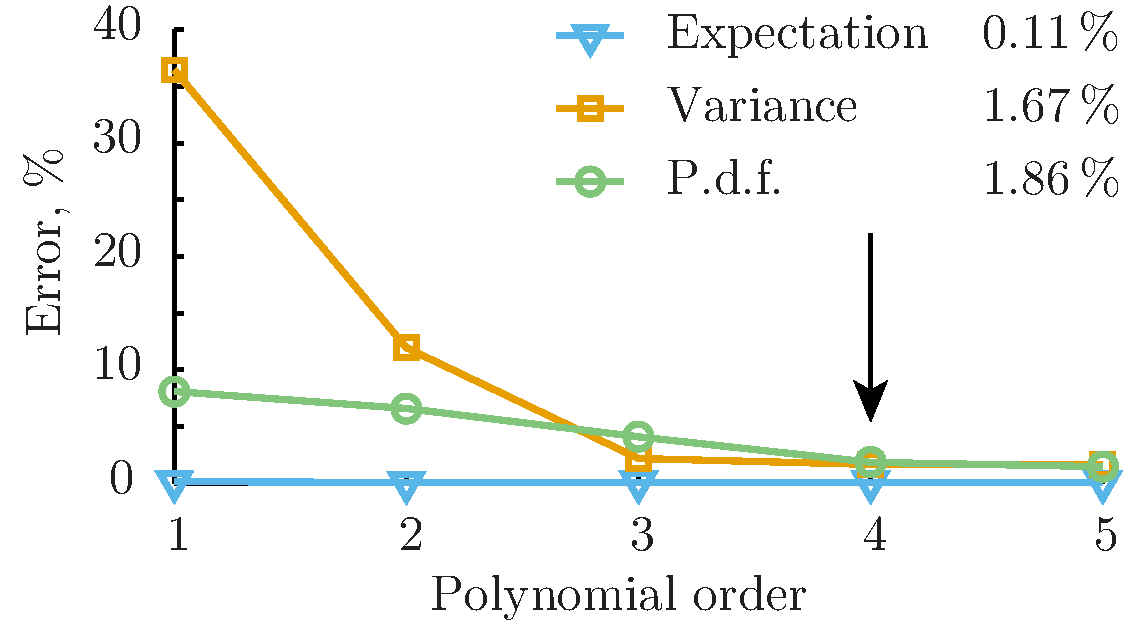
\includegraphics[width=1.0\columnwidth]{include/assets/accuracy.pdf}
  \caption{Errors of expectation, variance, and \pdf}
  \flabel{accuracy}
  \vspace{-1.6em}
\end{figure}

In this section, we report the results of the proposed framework for different configurations of the illustrative example in \sref{illustrative-example}.
All the experiments are conducted on a GNU/Linux machine with Intel Core i7 2.66~GHz and 8~GB of RAM.

Now we shall elaborate on the default configuration of our experimental setup, which, in the following subsections, will be adjusted according to the purpose of each particular experiment.
We consider a 45-nanometer technological process.
The effective channel length is assumed to have a nominal value of $17.5\,\text{nm}$ \cite{ptm} and a standard deviation of $2.25\,\text{nm}$ where the global and local variations are equally weighted.
Correlation matrices are computed according to \eref{correlation-function} where the length-scale parameters $\lCorrSE$ and $\lCorrOU$ are set to half the size of the square die.
In the model order reduction technique (see \sref{ie-uncertain-parameters}), the threshold parameter is set to 0.99 preserving 99\% of the variance of the data.
Dynamic power profiles involved in the experiments are based on simulations of randomly generated applications defined as directed acyclic task graphs.\footnote{In practice, dynamic power profiles are typically obtained \via\ an adequate simulator of the architecture of interest.}
The floorplans of the platforms are constructed in such a way that the processing elements form regular grids.\footnote{The task graphs of the applications, floorplans of the platforms, configuration of HotSpot, which was used to construct thermal RC circuits for our experiments, are available online at \cite{sources}.}
The time step of power and temperature traces is set to $1\,\text{ms}$ (see \sref{problem-formulation}), which is also the time step of the recurrence in \eref{pc-recurrence}.
As a comparison to our polynomial chaos (PC) expansions, we employ Monte Carlo (MC) sampling.
The MC approach is set up to preserve the whole variance of the problem, \ie, no model order reduction, and to solve \eref{fourier-system} directly using the Runge-Kutta formulae (the Dormand-Prince method) available in MATLAB \cite{matlab}.

Since the temperature part of PTA is the main contribution of this work, we shall focus on the assessment of temperature profiles.
Note, however, that the results for temperature allow one to implicitly draw reasonable conclusions regarding power since power is an intermediate step towards temperature, and any accuracy problems with respect to power are expected to propagate to temperature.
Also, since the temperature-driven studies \cite{juan2011, juan2012, huang2009, lee2013} work under the steady-state assumption (\cite{juan2011} is also limited to the maximal temperature, and \cite{huang2009} does not model the leakage-temperature interplay), a one-to-one comparison with our framework is not possible.

\subsection{Approximation Accuracy} \slabel{er-accuracy}
\begin{figure}
  \centering
  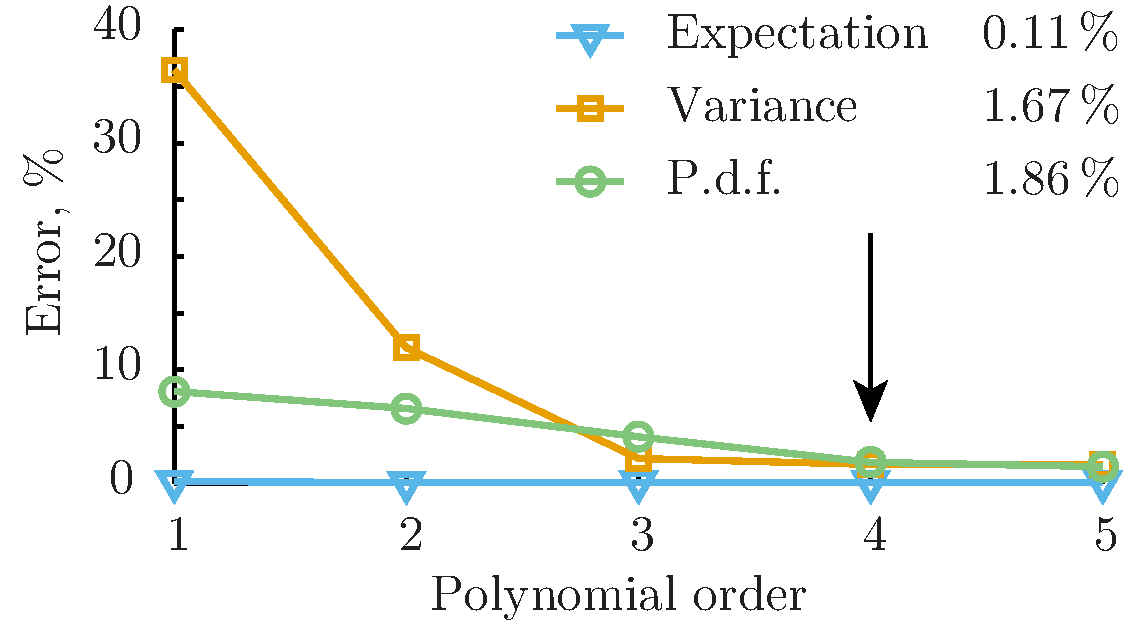
\includegraphics[width=1.0\columnwidth]{include/assets/accuracy.pdf}
  \caption{Errors of expectation, variance, and \pdf}
  \flabel{accuracy}
  \vspace{-1.6em}
\end{figure}


\subsection{Computational Speed} \slabel{er-speed}
\begin{table}[b]
  \vspace{-16pt}
  \centering
  \caption{Scaling with the number of processing elements $\cores$.}
  \begin{tabular*}{0.85\linewidth}{p{20pt}crrr}
    \toprule
    $\cores$ & $\vars$ & PC, seconds & MC, hours & Speedup, times \\
    \midrule
    $ 2$ & $2$ & $ 0.32$ & $31.24$ & $3.55 \times 10^5$ \\
    $ 4$ & $3$ & $ 0.45$ & $30.88$ & $2.46 \times 10^5$ \\
    $ 8$ & $4$ & $ 1.26$ & $31.44$ & $9.01 \times 10^4$ \\
    $16$ & $5$ & $ 6.55$ & $38.34$ & $2.11 \times 10^4$ \\
    $32$ & $6$ & $40.29$ & $41.58$ & $3.72 \times 10^3$ \\
    \bottomrule
  \end{tabular*}
  \tlabel{scaling-cores}
  \vspace{5pt}
  \caption{Scaling with the number of steps $\steps$.}
  \begin{tabular*}{0.85\linewidth}{p{42pt}rrr}
    \toprule
    $\steps$ & PC, seconds & MC, hours & Speedup, times \\
    \midrule
    $   10$ & $ 0.04$ & $   0.88$ & $8.19 \times 10^4$ \\
    $ 10^2$ & $ 0.06$ & $   3.12$ & $1.99 \times 10^5$ \\
    $ 10^3$ & $ 0.43$ & $  31.35$ & $2.65 \times 10^5$ \\
    $ 10^4$ & $ 4.35$ & $ 318.00$ & $2.63 \times 10^5$ \\
    $ 10^5$ & $42.23$ & $3110.29$ & $2.65 \times 10^5$ \\
    \bottomrule
  \end{tabular*}
  \tlabel{scaling-steps}
\end{table}

